\documentclass[10pt,a4paper]{article}
% ---------------------------------------------------------------- packages
\usepackage[T1]{fontenc}
\usepackage[utf8]{inputenc}
\usepackage{lmodern}
\usepackage{microtype}
\usepackage[a4paper,margin=2.1cm,top=2.0cm,bottom=2.2cm]{geometry}
\usepackage{graphicx}
\usepackage{booktabs}
\usepackage{tabularx}
\usepackage{array}
\usepackage{siunitx}
\usepackage{xcolor}
\usepackage{tikz}
\usetikzlibrary{arrows.meta,positioning,fit,calc,shapes.geometric}
\usepackage{enumitem}
\usepackage{amsmath,amssymb}
\usepackage[most]{tcolorbox}
\usepackage{caption}
\usepackage{titlesec}
\usepackage{float}
\usepackage{needspace}
\newcolumntype{Y}{>{\raggedright\arraybackslash}X}
\newcolumntype{P}[1]{>{\raggedright\arraybackslash}p{#1}}
\usepackage[hidelinks]{hyperref}

\setlist{nosep,leftmargin=1.3em,topsep=2pt}
\setlength{\parindent}{0pt}
\setlength{\parskip}{3pt}
\captionsetup{font=small,labelfont=bf,skip=4pt}
\sisetup{group-minimum-digits=5}
\renewcommand{\arraystretch}{1.12}
\titleformat{\section}{\large\bfseries\sffamily}{\thesection}{0.6em}{}
\titleformat{\subsection}{\normalsize\bfseries\sffamily}{\thesubsection}{0.6em}{}
\titlespacing*{\section}{0pt}{10pt}{4pt}
\titlespacing*{\subsection}{0pt}{8pt}{3pt}

% ---------------------------------------------------------------- colours
\definecolor{cblue}{HTML}{2A78D6}
\definecolor{corange}{HTML}{EB6834}
\definecolor{caqua}{HTML}{1BAF7A}
\definecolor{cyellow}{HTML}{EDA100}
\definecolor{inkgray}{HTML}{52514E}
\definecolor{gridgray}{HTML}{E1E0D9}
\definecolor{pendbg}{HTML}{FFF4E5}

% ---------------------------------------------------------------- macros
\newcommand{\tr}[2]{#1$\to$#2}                 % transition A->AA
\newcommand{\tA}{$\tau_A$}
\newcommand{\tB}{$\tau_B$}
\newcommand{\res}[1]{\texttt{\detokenize{#1}}}  % results path
\newcommand{\code}[1]{\texttt{\detokenize{#1}}}
\newcommand{\blk}[1]{\par\needspace{5\baselineskip}\smallskip{\sffamily\bfseries\color{inkgray}#1}\par}
\newcommand{\Q}{\blk{Question}}
\newcommand{\Setup}{\blk{Setup}}
\newcommand{\Result}{\blk{Result}}
\newcommand{\Comment}{\blk{Comment}}
\newenvironment{setup}{\par\footnotesize\noindent\tabularx{\linewidth}{@{}>{\bfseries\raggedright}p{2.85cm}Y@{}}\toprule}{\bottomrule\endtabularx\par}
\newtcolorbox{pending}[1][]{colback=pendbg,colframe=corange,boxrule=0.8pt,arc=2pt,
  left=6pt,right=6pt,top=4pt,bottom=4pt,fontupper=\small,
  title={\sffamily\bfseries Result pending --- #1},coltitle=white,colbacktitle=corange}
\newtcolorbox{keybox}{colback=gridgray!35,colframe=gridgray!90!black,boxrule=0.5pt,arc=2pt,
  left=5pt,right=5pt,top=3pt,bottom=3pt,fontupper=\small}
% include a figure if make_figures.py produced it, otherwise a pending box
\newcommand{\figorpending}[4]{%
  \IfFileExists{figures/#1.pdf}{%
    \begin{figure}[H]\centering\includegraphics[width=#2\linewidth]{figures/#1}\caption{#3}\label{fig:#1}\end{figure}}%
  {\begin{pending}[sweep running / planned]#4\end{pending}}}
% same, but silent when the figure is missing (second panel of a pending result)
\newcommand{\figorskip}[3]{\IfFileExists{figures/#1.pdf}{\figorpending{#1}{#2}{#3}{}}{}}

\hypersetup{pdftitle={BIO-SBI: simulation experiments report},pdfauthor={BIO-SBI}}

\begin{document}

% ====================================================================== title
\begin{titlepage}
\centering
\vspace*{3cm}
{\sffamily\Huge\bfseries BIO-SBI\par}
\vspace{0.5cm}
{\sffamily\LARGE Simulation experiments for planning\\ organoid lineage experiments\par}
\vspace{1.2cm}
{\large Two-type branching models (LGR5$^+$ = A, KRT20$^+$ = B),\\ neural posterior estimation, identifiability and robustness\par}
\vspace{1.5cm}
\begin{tabular}{ll}
Status of results & 5 November 2026 \\
Repository & \code{BIO-SBI}, branch \code{main}, commit \code{5a1b926} \\
Data & synthetic only (no measured data used) \\
Audience & group planning the wet-lab organoid experiments \\
\end{tabular}
\vfill
\begin{minipage}{0.82\linewidth}\small
\textbf{How to read this report.} The executive summary (p.~\pageref{sec:summary}) is self-contained.
Section~\ref{sec:methods} defines the model and every diagnostic.
Each experiment section has the same four parts: \emph{Question}, \emph{Setup}, \emph{Result}, \emph{Comment}.
Orange boxes mark experiments whose sweeps are still running or planned.
Parameters: A$\to$AA etc.\ are outcome probabilities per cell event; \tA, \tB{} are mean cell lifetimes (Bellman--Harris only).
\end{minipage}
\end{titlepage}

% ====================================================================== summary
\section*{Executive summary}\label{sec:summary}
\addcontentsline{toc}{section}{Executive summary}

\textbf{Scope.} 15 finished experiments (616 runs), all on synthetic data from one reference parameter vector $\theta^\star$ (Table~\ref{tab:truth}), 5 seeds per setting. Galton--Watson (GW, time in generations) and Bellman--Harris (BH, time in hours; real-like design = days 6 and 10 = 144/240\,h with 165/101 organoids).

\subsection*{Key findings}
\begin{enumerate}[leftmargin=1.4em]
\item \textbf{The well-specified GW model is recovered at the real-like design}: MAE 0.033 over the 9 outcome probabilities, mean contraction 0.89, A$\to$AA 0.52 (truth 0.55) --- provided B's divisions are fixed to 0 (\S\ref{sec:e1a}).
\item \textbf{B's row is prior-dominated if all transitions are free} (E0): B$\to$A = 0.20 vs truth 0.80, contraction $\le 0$, at 5k--50k simulations, every dataset, every design. Cause: the uniform Dirichlet prior puts 0.03\% mass above 0.8; a flat prior gives 0.53 (4/5 covered). Switching and division differ only in clone-size variability: a shift of 0.05 in B$\to$A is detectable at 512 clones per endpoint (C2ST 0.84), not at 32 (0.57).
\item \textbf{Endpoints matter more than organoids.} GW: 3 endpoints $\times$ 128 halve the error of 1 endpoint $\times$ 384 (MAE 0.028 vs 0.058). BH (E4): days \{4,6,10\} beat every other set at every size; mean contraction 0.50 $\to$ 0.79 at 512 organoids/endpoint; day 10 alone plateaus at 0.50.
\item \textbf{BH baseline bias = lifetime/self-renewal ridge.} Even well specified, BH estimates A$\to$AA $\approx$ 0.32 (truth 0.55) and \tA{} $\approx$ 16\,h (truth 20\,h), 0/5 covered, at every design from 16 to 512 organoids. Fixing lifetimes to the truth gives 0.51 (5/5), MAE 0.109 $\to$ 0.059 (\S\ref{sec:ridge}). More organoids do not help.
\item \textbf{Most misspecifications are silent} (Fig.~\ref{fig:detectability}). In all BH error experiments the PPC stays $\le 0.033$ (well-specified: 0--0.008) except two cases: both death rates fixed wrong (0.096) and a global lifetime longer than A's (0.35--0.51, support mass $\approx 0$). Shifts up to $\approx$\,2 posterior sd go unnoticed.
\item \textbf{Size of the tested errors (BH, vs well-specified control):}
  \begin{itemize}
  \item founders 50\% B: A$\to$AB $-0.11$, \tB{} $+4$\,h; 40\% multi-cell clones: \tA{} $-1.8$\,h, B$\to$A $-0.07$;
  \item death fixed wrong: B death 0.4 (true 0.1) $\Rightarrow$ B$\to$A $-0.19$ (0/5 covered), A$\to$AB $+0.17$;
  \item mis-typing ignored, $e=0.2$: A$\to$AB $+0.09$, A$\to$AA $-0.06$ ($\le$\,0.7 sd); modelled: no bias, A$\to$AB contraction 0.30 $\to -0.22$;
  \item lifetime CV 0.18--0.5: harmless ($\le$\,0.035); exponential (CV 1): A$\to$AA $+0.16$, B$\to$A $-0.18$, \tA{} $-3.7$\,h;
  \item quiescence (A persist) not identifiable: posterior 0.12--0.14 for truths 0.03--0.30.
  \end{itemize}
\item \textbf{Founder mix and founder size cannot be learned} from endpoint counts in BH (contraction $\le 0.12$); in GW the founder A share is partly informed but compressed (0.68 for truth 0.5, 0.78 for 1.0).
\item \textbf{Observed-organoid fraction} (detected/seeded): 0.94--0.95 at $\theta^\star$; dominated by A death (0.3 $\Rightarrow$ 0.54--0.58); GW exact and BH simulated agree within $\approx$\,0.03; A and B death trade off (one constraint, not two).
\item \textbf{Hidden third type ignored (GW, E2c)}: PPC 0.17--0.41 and support mass 0.01--0.16, i.e.\ flagged --- but this sweep has no well-specified control and its truth lies far in the prior tail, so the flag cannot yet be attributed to C alone.
\end{enumerate}

\subsection*{Recommendations for the wet-lab design}
\begin{itemize}
\item \textbf{Endpoints:} at least 2, preferably 3 including an early one --- e.g.\ days 4, 6, 10. A single day-10 endpoint is the weakest design.
\item \textbf{Organoids:} $\ge 128$ per endpoint (BH contraction 0.71 at \{4,6,10\}$\times$128; 0.77 at 256). A$\to$BB needs $\ge 64$, B death $\ge 128$, A$\to$AB $\ge 256$ per endpoint (BH, days 4/6/10).
\item \textbf{Measure independently:}
  \begin{enumerate}[label=(\alph*)]
  \item \emph{A (LGR5$^+$) division time} by live imaging --- the single most valuable measurement; per type, not pooled (a pooled value longer than A's makes the model fail; shorter biases silently);
  \item \emph{number of organoids seeded per well} (gives the observed fraction, sensitive to A death);
  \item \emph{cell-cycle variability}: only whether CV is $<0.5$ or near-exponential;
  \item \emph{mis-typing rate} (2D vs 3D comparison), to pass to the model;
  \item \emph{founder composition at seeding} and \emph{quiescence} (e.g.\ Ki67) if they matter biologically --- the counts cannot provide them;
  \item \emph{apoptosis} only if death rates are to be fixed; otherwise keep them free.
  \end{enumerate}
\item \textbf{Biological constraints help more than data}: B divisions = 0 (if KRT20$^+$ cells do not divide) is what makes B$\to$A identifiable.
\end{itemize}

\subsection*{Methodological lessons}
\begin{itemize}
\item \textbf{Prior tails}: a truth with $<$\,2\% prior mass (B$\to$A = 0.8, A$\to$AA = 0.55 under uniform Dirichlet) is pulled to the prior, and SBC still looks fine. Report prior quantiles of the truth; check prior sensitivity.
\item \textbf{Ridges}: endpoint counts fix the growth rate; lifetime, self-renewal and quiescence trade off along it (posterior corr.\ $+0.7$, $-0.6$). The prior picks the point.
\item \textbf{Compare with paired controls}, not with the truth (BH baseline is biased); 5 seeds resolve shifts of $\approx$\,0.02--0.03 (probabilities) and 0.5--1.5\,h.
\item \textbf{Diagnostics}: SBC checks the inference model only and cannot see misspecification; PPC and support mass are relative checks; support mass $\approx 0$ = the model cannot explain the data (numbers from such runs are not estimates).
\end{itemize}

\textbf{Still running / planned} (Part~\ref{part:pending}): GW halves of E4, E1c, E1a founder number, E2a/E2b; E2c with C modelled (free / trajectory-constrained); X1 methods comparison, X2 seed spread, X3 GW vs BH, X4 combined errors, R real CRC0322 data.

\figorpending{detectability}{0.78}{Detectability of BH misspecifications. Each point is one misspecified setting (mean of 5 seeds): largest shift of a posterior mean from its paired well-specified control, in units of the control's posterior sd, against the PPC. Grey band = PPC range of well-specified runs. Crosses: global lifetime $T>\tau_A$ (support mass $\approx 0$).}{Detectability scatter.}

\clearpage
{\setcounter{tocdepth}{1}\tableofcontents}
\clearpage

% ====================================================================== methods
\section{Methods overview}\label{sec:methods}

\subsection{Model}
\begin{minipage}[t]{0.50\linewidth}
\vspace{0pt}
\begin{itemize}
\item \textbf{Two cell types}: A = LGR5$^+$ (stem-like), B = KRT20$^+$ (differentiated).
\item \textbf{One event per cell}: a cell is replaced by 0, 1 or 2 daughters. Outcomes of A: death, persist (stays, no division), A$\to$B (switch), divisions A$\to$AA, A$\to$AB, A$\to$BB. B mirrors A.
\item \textbf{Parameters}: one probability simplex per type; Dirichlet(1,\dots,1) prior (uniform).
\item \textbf{Laws}: \code{two_type} = all 12 outcomes free (10 free params); \code{reversible_ab} = B divisions fixed to 0 (B: death, persist, B$\to$A; 7 free) --- the baseline of every experiment after E0.
\item \textbf{Founders}: a clone (organoid) starts from $N$ cells ($P(N{=}n)$ = \code{founder_size}) of i.i.d.\ type (\code{founder}); baseline: one A cell.
\end{itemize}
\end{minipage}\hfill
\begin{minipage}[t]{0.47\linewidth}
\vspace{0pt}\centering
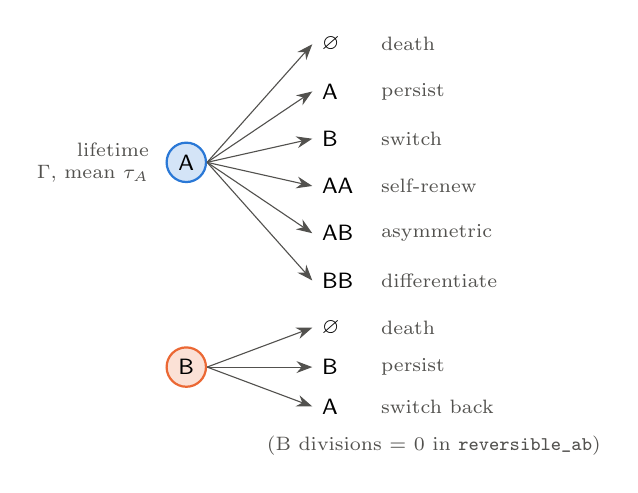
\begin{tikzpicture}[font=\footnotesize\sffamily,
  cA/.style={circle,draw=cblue,fill=cblue!20,thick,minimum size=5mm,inner sep=0},
  cB/.style={circle,draw=corange,fill=corange!20,thick,minimum size=5mm,inner sep=0},
  arr/.style={-{Stealth[length=2mm]},inkgray}]
\node[cA] (a) at (0,0) {A};
\node[font=\scriptsize,inkgray,align=right,anchor=east] at (-0.35,0) {lifetime\\$\Gamma$, mean $\tau_A$};
\foreach \y/\lab/\d [count=\i] in {1.5/death/{$\varnothing$},0.9/persist/{A},0.3/switch/{B},-0.3/self-renew/{AA},-0.9/asymmetric/{AB},-1.5/differentiate/{BB}}{
  \node[anchor=west] (o\i) at (1.6,\y) {\d};
  \node[anchor=west,inkgray,font=\scriptsize] at (2.35,\y) {\lab};
  \draw[arr] (a.east) -- (o\i.west);
}
\node[cB] (b) at (0,-2.6) {B};
\foreach \y/\lab/\d [count=\i] in {-2.1/death/{$\varnothing$},-2.6/persist/{B},-3.1/switch back/{A}}{
  \node[anchor=west] (p\i) at (1.6,\y) {\d};
  \node[anchor=west,inkgray,font=\scriptsize] at (2.35,\y) {\lab};
  \draw[arr] (b.east) -- (p\i.west);
}
\node[font=\scriptsize,inkgray,anchor=west] at (0.9,-3.6) {(B divisions = 0 in \code{reversible_ab})};
\end{tikzpicture}
\end{minipage}

\begin{table}[H]\centering\footnotesize
\caption{Reference truth $\theta^\star$ used by every experiment unless stated (\code{law.reference}); one founder cell of type A. Prior probability of exceeding the truth under the uniform Dirichlet: A$\to$AA 1.8\%; B$\to$A 0.03\% (\code{two_type}) or 4\% (\code{reversible_ab}).}\label{tab:truth}
\begin{tabular}{@{}lrrrrrrl@{}}\toprule
Type & death & persist & switch & $\to$AA & $\to$AB & $\to$BB & mean lifetime (BH) \\\midrule
A & 0.03 & 0.03 & 0.05 (A$\to$B) & \textbf{0.55} & 0.05 & 0.29 & \tA{} = 20\,h \\
B & 0.10 & 0.10 & \textbf{0.80} (B$\to$A) & 0 & 0 & 0 & \tB{} = 30\,h \\\bottomrule
\multicolumn{8}{@{}l}{BH lifetimes: Gamma, shape 8 (CV 0.35). GW: one event per generation.}
\end{tabular}
\end{table}

\subsection{Two simulators}
\begin{center}\footnotesize
\begin{tabularx}{\linewidth}{@{}P{2.5cm}YY@{}}\toprule
 & \textbf{Galton--Watson (GW)} & \textbf{Bellman--Harris (BH)} \\\midrule
Time & synchronous generations; endpoints in \emph{generations} (real-like: 6 and 10) & continuous; Gamma lifetimes per type; endpoints in \emph{hours} (real-like: 144 and 240\,h = days 6, 10) \\
Extra parameters & none & \tA, \tB{} (log-uniform prior); shape fixed (8) \\
Sampling & exact detection-conditioned sampler; exact observed fraction & forward simulation + rejection; observed fraction estimated \\
Cost & cheap & slower (rejection sampling; P0 timing not run) \\\bottomrule
\end{tabularx}
\end{center}
GW and BH share the outcome law but not the time unit; a GW generation is \emph{not} a day (X3 needs a mapping).

\subsection{Observation, data model and inference model}
\begin{itemize}
\item \textbf{Observation}: biology $\to$ capture (Binomial per true type) $\to$ labelling (confusion matrix true type $\times$ label; may be rectangular, e.g.\ hidden C read as A with prob.\ $q$) $\to$ selection of \emph{recovered} clones ($\ge 1$ detected cell). Baseline: perfect capture and typing.
\item \textbf{Data}: per endpoint, A and B counts of each recovered organoid. Endpoints are destructive: different organoids per endpoint.
\item \textbf{Misspecification}: the reference data come from a separate \emph{data model} (\code{data.simulator}, \code{data.law}, \code{data.observation}, with seed \code{data_seed}); the \emph{inference model} defines prior, training simulations and checks. An error is tested by changing one side only.
\end{itemize}

\subsection{Inference}
\begin{itemize}
\item \textbf{NPE} (\code{sbi} 0.27, neural spline flow, 5 transforms, width 64), amortised, 1 round; sequential NPE (SNPE) only in E0.
\item \textbf{Summaries} (\code{moments}): per endpoint, mean, sd, quantiles of $\log(1+n)$ for A, B, total; fraction of clones containing each type; fraction empty; correlation of log counts.
\item \textbf{Budgets}: \code{dev} = 5\,000 simulations (all BH and most GW error experiments); 20\,000 for E0/design comparison; E0 also 50\,000. E0 showed 5k$\to$50k does not change recovery. Per run: 2\,000 posterior samples, SBC on 200 prior draws, PPC with 200 datasets.
\item \textbf{Parameterisation}: stick-breaking of each simplex (exact Dirichlet reparameterisation).
\end{itemize}

\subsection{Pipeline and experiment logic}
\begin{center}
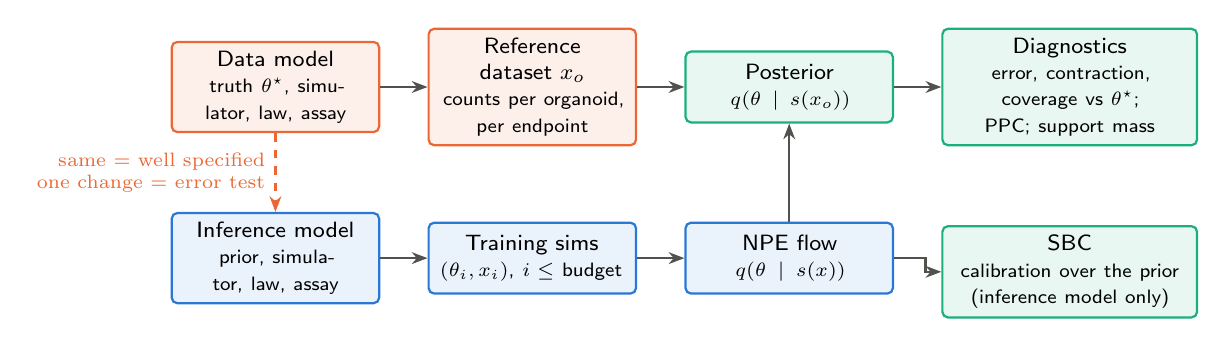
\begin{tikzpicture}[font=\footnotesize\sffamily, node distance=4mm and 6mm,
  box/.style={draw=#1,fill=#1!10,rounded corners=2pt,thick,align=center,minimum height=9mm,text width=24mm},
  box/.default=cblue,
  arr/.style={-{Stealth[length=2mm]},thick,inkgray}]
\node[box=corange] (dm) {Data model\\\scriptsize truth $\theta^\star$, simulator, law, assay};
\node[box=corange,right=of dm] (xo) {Reference dataset $x_o$\\\scriptsize counts per organoid, per endpoint};
\node[box=cblue,below=10mm of dm] (im) {Inference model\\\scriptsize prior, simulator, law, assay};
\node[box=cblue,right=of im] (sims) {Training sims\\\scriptsize $(\theta_i, x_i)$, $i\le$ budget};
\node[box=cblue,right=of sims] (npe) {NPE flow\\\scriptsize $q(\theta\mid s(x))$};
\node[box=caqua,right=of xo] (post) {Posterior\\\scriptsize $q(\theta\mid s(x_o))$};
\node[box=caqua,right=of post,text width=30mm] (diag) {Diagnostics\\\scriptsize error, contraction, coverage vs $\theta^\star$; PPC; support mass};
\node[box=caqua,below=10mm of diag,text width=30mm] (sbc) {SBC\\\scriptsize calibration over the prior (inference model only)};
\draw[arr] (dm) -- (xo);
\draw[arr] (im) -- (sims);
\draw[arr] (sims) -- (npe);
\draw[arr] (npe) -- (post);
\draw[arr] (xo) -- (post);
\draw[arr] (post) -- (diag);
\draw[arr] (npe.east) -- ++(4mm,0) |- (sbc.west);
\draw[arr,dashed,corange] (dm.south) -- node[left,font=\scriptsize,align=right]{same = well specified\\one change = error test} (im.north);
\end{tikzpicture}
\end{center}
\textbf{Experiment logic}: vary one error on the data side (or one assumption on the inference side), keep everything else at the baseline, and compare with the \emph{well-specified control of the same sweep} (same seeds, same datasets; often the same trained network, so differences are paired by seed).

\subsection{Diagnostics and how to read them}
\begin{center}\footnotesize
\begin{tabularx}{\linewidth}{@{}P{3.0cm}YY@{}}\toprule
\textbf{Metric} & \textbf{Definition} & \textbf{How to read} \\\midrule
Posterior mean / error & mean of 2\,000 posterior samples; $|$mean $-$ truth$|$. MAE over probabilities only (\code{mae_probabilities}); lifetimes separately & compare misspecified vs control; ``shift'' = difference of posterior means, paired by seed, $\pm$ paired SE over 5 seeds \\
Contraction & $1-\mathrm{Var}_\text{post}/\mathrm{Var}_\text{prior}$ & 0 = data uninformative; $<0$ = wider than prior; $>0.5$ = informative \\
90\% coverage across seeds & number of seeds (of 5) whose 90\% credible interval contains the truth & 4--5/5 expected; 0/5 with high contraction = confident bias \\
SBC coverage error & mean $|$empirical $-$ nominal$|$ coverage of central intervals (50--95\%) over 200 prior draws & $\le 0.03$ = calibrated. Averages over the prior: blind to tail truths and to misspecification \\
PPC fraction outside 95\% & share of summary features whose observed value lies outside the 95\% posterior predictive interval & well specified: 0--0.03. Higher = the model cannot reproduce the data. Relative check \\
Posterior support mass & share of the NPE posterior inside the prior support & well specified $\approx$\,0.5--0.9 (not 1). $\approx 0$ = model cannot explain the data; few/no samples, not an estimate \\
Recovered (TODO criterion) & contraction $>0.5$, $|$error$|<0.05$, coverage $\ge 4/5$ & used for ``organoids needed'' (E4) \\\bottomrule
\end{tabularx}
\end{center}

\begin{keybox}
\textbf{Reading rules used throughout.}
(1) \emph{BH baseline bias}: well-specified BH runs give A$\to$AA $\approx$ 0.32 and \tA{} $\approx$ 16\,h (truth 0.55, 20\,h); BH misspecified arms are compared with their control, never with the truth.
(2) With all transitions free, B's row is prior-dominated (E0).
(3) A misspecification that raises neither PPC nor lowers support mass is \emph{undetectable from the fit}.
(4) 5 seeds per setting: effects below $\approx$\,2 paired SE are not resolved.
(5) Wall times in run metrics were measured under heavy contention; only the device benchmark (\S\ref{sec:gpu}) measures speed.
\end{keybox}

% ====================================================================== PART I
\clearpage
\part{Finished experiments}\label{part:finished}

% ---------------------------------------------------------------------- E0
\section{E0 --- Identifiability of B's row (GW)}\label{sec:e0}
\Q
With all transitions free, B$\to$A (true 0.80) came out at $\approx$\,0.2. Is this under-training, one bad dataset, miscalibration, a prior-tail effect, or non-identifiability (switching vs division)?
\Setup
\begin{setup}
Simulator & Galton--Watson, perfect observation \\
Law (free) & \code{two_type} (10) vs \code{reversible_ab} (7; B divisions fixed to their true 0) \\
Data vs inference & well specified (same $\theta^\star$, Table~\ref{tab:truth}) \\
Design & generations 4, 8, 12 $\times$ 32 clones (96 organoids) \\
Inference / budget & NPE amortised 5k, 20k, 50k; SNPE 4 rounds $\times$ 5k; \code{two_type} with flat prior on B$\to$A (Beta(1,1)), 20k \\
Seeds / runs & 5 / 40 (+ direct checks: C2ST of mean-preserving alternatives, 500 datasets per side) \\
Varied & law, budget, method, prior \\
Folder & \res{results/b_row/} (\res{distinguish.csv}, \res{truth_vs_posterior_20k*.csv}) \\
\end{setup}
\Result
\figorpending{e0_bto_a}{1.0}{B$\to$A posterior mean $\pm$ sd per seed. Orange: all B outcomes free (uniform Dirichlet; squares: SNPE). Green: flat prior on B$\to$A. Blue: B divisions fixed to 0.}{E0 figure.}
\begin{center}\footnotesize
\begin{tabular}{@{}llrrrrr@{}}\toprule
Law & Training & B$\to$A mean & post.\ sd & contraction & covered & MAE (all) \\\midrule
\code{two_type} & 5k / 20k / 50k & 0.20 / 0.21 / 0.22 & 0.14--0.15 & $-0.03$ / $-0.13$ / $-0.18$ & 0/15 & 0.14 \\
\code{two_type} & SNPE 4$\times$5k & 0.21 & 0.16 & $-0.22$ & 0/5 & 0.14 \\
\code{two_type}, flat prior & 20k & 0.53 & 0.21 & 0.46 & 4/5 & 0.10 \\
\code{reversible_ab} & 5k / 20k / 50k & 0.72 / 0.71 / 0.70 & 0.13--0.14 & 0.67 / 0.71 / 0.69 & 15/15 & 0.05 \\\bottomrule
\end{tabular}
\end{center}
\begin{minipage}[c]{0.46\linewidth}
\figorpending{e0_c2st}{1.0}{C2ST accuracy separating the truth from a mean-preserving alternative (B$\to$AA $=a$, B$\to$A $=0.8-2a$, B death $=0.1+a$). 0.5 = indistinguishable.}{C2ST heat map.}
\end{minipage}\hfill
\begin{minipage}[c]{0.5\linewidth}\footnotesize
\begin{itemize}
\item SBC coverage error 0.02--0.04 in every arm (looks calibrated).
\item PPC $\le 0.014$ in every arm.
\item Flat prior: corr(B$\to$A, B$\to$AA) $= -0.67$; SBC fails (0.069) for B's other coordinates (concentration 0.2), not for B$\to$A.
\item Truth-vs-posterior C2ST: inconclusive (0.62--0.95 in both laws).
\end{itemize}
\end{minipage}
\Comment
\begin{itemize}
\item Under-training, dataset and calibration are ruled out: 10$\times$ more simulations, 5 datasets, SBC all unchanged.
\item Main cause = prior tail: B$\to$A $\sim$ Beta(1,5), P($>0.8$) = 0.03\% ($\approx$\,15 of 50k training simulations). SNPE cannot help: round 0 is already prior-like.
\item Data weakly confound switching with division: even with a flat prior the posterior is wide (sd 0.21) and anti-correlated with B$\to$AA. They differ only in clone-size variability; 128--512 clones/endpoint make moderate differences detectable.
\item Consequence: fix what biology allows (B divisions = 0 $\Rightarrow$ B$\to$A $\approx$ 0.70, contraction 0.7); otherwise report prior sensitivity. All later experiments use \code{reversible_ab}.
\end{itemize}

% ---------------------------------------------------------------------- design
\section{Design comparison --- one vs three endpoints (GW)}\label{sec:design}
\Q Which planned design identifies the model best, and is it the number of time points or the number of organoids that matters?
\Setup
\begin{setup}
Simulator & Galton--Watson, perfect observation \\
Law (free) & \code{two_type} (10) and \code{reversible_ab} (7) \\
Data vs inference & well specified, $\theta^\star$ \\
Design & \code{single_128}: gen.\ 12 $\times$ 128; \code{three_128}: gen.\ 4, 8, 12 $\times$ 128; \code{single_384}: gen.\ 12 $\times$ 384; reference \code{three_32} (from E0) \\
Inference / budget & NPE amortised, 20k \\
Seeds / runs & 5 / 30 (+ 10 reference runs from E0) \\
Varied & design $\times$ law \\
Folder & \res{results/design_comparison/} \\
\end{setup}
\Result
\figorpending{design_comparison}{1.0}{Left, centre: MAE and mean contraction per design (mean $\pm$ sd over 5 seeds); total organoids in brackets. Right: contraction per parameter, B divisions fixed.}{Design figure.}
\begin{center}\footnotesize
\begin{tabular}{@{}lrrrrrrr@{}}\toprule
Design (\code{reversible_ab}) & organoids & MAE & contraction & 90\% cov. & B$\to$A & B$\to$A contr. & PPC \\\midrule
1 $\times$ 128 & 128 & 0.079 & 0.77 & 0.87 & 0.61 $\pm$ 0.17 & 0.50 & 0.000 \\
3 $\times$ 32 & 96 & 0.052 & 0.86 & 0.96 & 0.71 $\pm$ 0.13 & 0.71 & 0.008 \\
1 $\times$ 384 & 384 & 0.058 & 0.84 & 0.93 & 0.67 $\pm$ 0.12 & 0.72 & 0.000 \\
\textbf{3 $\times$ 128} & 384 & \textbf{0.028} & \textbf{0.93} & 0.93 & \textbf{0.78 $\pm$ 0.09} & \textbf{0.87} & 0.031 \\\midrule
\code{two_type}, any design & 96--384 & 0.13--0.15 & 0.45--0.53 & 0.69--0.78 & 0.18--0.25 & $\le -0.03$ & $\le$ 0.014 \\\bottomrule
\end{tabular}
\end{center}
\Comment
\begin{itemize}
\item At equal organoids, 3 endpoints halve the error of 1 (0.028 vs 0.058). Gains are in dynamics: A$\to$AB contraction 0.90 vs 0.60, B$\to$A 0.87 vs 0.72.
\item 96 organoids over 3 endpoints $\approx$ 384 at one endpoint.
\item With all transitions free no design recovers B's row (B$\to$A contraction $\le 0$) --- consistent with E0.
\item Calibration fine everywhere (SBC 0.02--0.03). Caveat: GW, one truth, generations not days.
\end{itemize}

% ---------------------------------------------------------------------- E4 BH
\section{E4 --- Amount of data: organoids and endpoints (BH)}\label{sec:e4}
\Q How do contraction and error depend on organoids per endpoint (16--512) and on the measured days? What is the minimum number to recover each parameter?
\Setup
\begin{setup}
Simulator & Bellman--Harris, Gamma lifetimes shape 8 \\
Law (free) & \code{reversible_ab}: 7 probabilities + \tA, \tB{} (9) \\
Data vs inference & well specified, $\theta^\star$ \\
Design & clones per endpoint $\in \{16,32,64,128,256,512\}$ $\times$ endpoints \{240\}, \{144, 240\}, \{144, 240, 336\}, \{96, 144, 240\}\,h = days \{10\}, \{6,10\}, \{6,10,14\}, \{4,6,10\} \\
Inference / budget & NPE amortised, 5k \\
Seeds / runs & 5 / 120 \\
Varied & clones $\times$ endpoint set \\
Folder & \res{results/e4/bh/} \\
\end{setup}
\Result
\figorpending{e4_bh_heat}{1.0}{Mean contraction and MAE of the 7 outcome probabilities (mean over 5 seeds).}{E4 BH heat map.}
\figorpending{e4_bh_params}{1.0}{Posterior means (mean $\pm$ SE over seeds) vs organoids per endpoint, one line per endpoint set; dashed = truth.}{E4 BH parameter lines.}
\begin{center}\footnotesize
\textbf{Minimum organoids per endpoint for ``recovered''} (contraction $>0.5$, $|$error$|<0.05$, $\ge$\,4/5 covered); --- = not reached at 512.\\[2pt]
\begin{tabular}{@{}lrrrr@{}}\toprule
Parameter & day 10 & days 6, 10 & days 6, 10, 14 & days 4, 6, 10 \\\midrule
A death, A$\to$B (small truths) & 16 & 16 & 16 & 16 \\
A$\to$BB & --- & 512 & 256 & \textbf{64} \\
B death & --- & 256 & 256 & \textbf{128} \\
A$\to$AB & --- & --- & --- & \textbf{256} \\
A$\to$AA, A persist, B persist, B$\to$A & --- & --- & --- & --- \\
\tA, \tB{} (biased: \tA{} 15--17\,h, 0/5 covered) & --- & --- & --- & --- \\\bottomrule
\end{tabular}
\end{center}
\Comment
\begin{itemize}
\item An early endpoint (day 4) helps most; day 10 alone plateaus (contraction 0.37 $\to$ 0.50 from 16 to 512).
\item With several endpoints more organoids keep helping (MAE 0.114 $\to$ 0.060 for days 4/6/10); B$\to$A rises 0.59 $\to$ 0.73.
\item A$\to$AA (0.29--0.39) and \tA{} (15--17\,h) are never recovered; coverage falls to 0 as posteriors narrow on the wrong values: the ridge (\S\ref{sec:ridge}), not lack of data.
\item ``Recovered'' for A death / A$\to$B is easy because the truths are small ($|$error$|<0.05$ is loose there).
\item Caveat: one truth, perfect assay, single A founders, 5k simulations; GW half pending (\S\ref{sec:p-e4gw}).
\end{itemize}

% ---------------------------------------------------------------------- ridge
\section{BH ridge --- lifetime vs self-renewal}\label{sec:ridge}
\Q Is the BH baseline bias (A$\to$AA $\approx$ 0.32, \tA{} $\approx$ 16\,h) a ridge on which endpoint counts fix only a combination of lifetime and self-renewal, with the prior picking the point?
\Setup
\begin{setup}
Simulator & Bellman--Harris, shape 8 \\
Law (free) & control: \code{reversible_ab} (9); lifetimes fixed: 7; flat prior: 9 \\
Data vs inference & data always $\theta^\star$; only the inference model changes \\
Design & real-like: 144/240\,h $\times$ 165/101 \\
Inference / budget & NPE amortised, 5k \\
Arms & control (from E3b, shape 8); \tA=20, \tB=30\,h fixed; flat prior on A$\to$AA (concentration 1 vs 0.2 for A's other outcomes: A$\to$AA $\sim$ Beta(1,1)) \\
Seeds / runs & 5 / 10 (+5 control) \\
Folder & \res{results/bh_ridge/} (control: \res{results/e3b/*lifetime_shape=8*}) \\
\end{setup}
\Result
\figorpending{bh_ridge}{1.0}{(a) A$\to$AA posterior pooled over 5 seeds; dotted: uniform-Dirichlet prior Beta(1,5). (b) Joint posterior of A$\to$AA and \tA{} (blue: control; green: flat prior); star = truth. (c) Per-seed means $\pm$ sd; dashed = truth.}{Ridge figure.}
\begin{center}\footnotesize
\begin{tabular}{@{}lccc@{}}\toprule
 & Control & Lifetimes fixed & Flat prior \\\midrule
A$\to$AA (0.55) & 0.32 $\pm$ 0.10, 0/5, contr.\ 0.52 & \textbf{0.51 $\pm$ 0.04, 5/5, 0.93} & 0.46 $\pm$ 0.12, 5/5, 0.83 \\
A$\to$AB (0.05) & 0.23, 3/5 & 0.17, 2/5 & 0.20, 5/5, contr.\ 0.00 \\
B$\to$A (0.80) & 0.63, 5/5 & 0.68, 5/5 & 0.46, 3/5 \\
\tA{} (20\,h) & 15.9 $\pm$ 1.9, 0/5 & fixed & 18.9 $\pm$ 2.2, 5/5 \\
MAE (probabilities) & 0.109 & \textbf{0.059} & 0.117 \\
SBC error / PPC / support & 0.025 / 0.008 / n/r & 0.031 / 0.025 / 0.65 & 0.079 / 0.000 / 0.51 \\\bottomrule
\end{tabular}
\end{center}
\Comment
\begin{itemize}
\item Ridge confirmed: posterior corr(A$\to$AA, \tA) $\approx +0.7$ (E3c). Removing the lifetime degree of freedom recovers self-renewal and halves the error.
\item The prior chose the point: only 1.8\% of uniform-Dirichlet mass lies above 0.55. A flat prior re-centres (5/5 covered) but stays wide, degrades B$\to$A and calibration: not a fix.
\item GW has no lifetimes and no ridge: the GW control at the same design gives A$\to$AA 0.52 (\S\ref{sec:e1a}).
\item Consequence: measure A's division time (live imaging) or use it as an informative prior; otherwise report BH results with prior sensitivity.
\end{itemize}

% ---------------------------------------------------------------------- E1a type
\section{E1a --- Wrong founder type (organoid death as initial conditions; BH and GW)}\label{sec:e1a}
\Q If some organoids are founded by B cells (fraction $1-f$) but the model assumes A founders, are the dynamics (A, B rows) biased? Does inferring the founder mix help?
\Setup
\begin{setup}
Simulator & Bellman--Harris (shape 8) and Galton--Watson \\
Law (free) & \code{reversible_ab}: BH 9, GW 7; inferred arm adds \code{founder.A} (Dirichlet(1,1)) \\
Data model & founder A with prob.\ $f \in \{1, 0.9, 0.7, 0.5\}$, else B; dynamics $\theta^\star$ \\
Inference model & fixed arm: founder = A (wrong for $f<1$); inferred arm: founder share free \\
Design & real-like: BH 144/240\,h, GW generations 6/10; 165/101 organoids \\
Inference / budget & NPE amortised, 5k \\
Seeds / runs & 5 / 80 (4 $f$ $\times$ 2 arms $\times$ 2 simulators) \\
Control & $f=1$ of the same arm (same trained network per seed: paired shifts) \\
Folder & \res{results/e1a/founder_type/{fixed,inferred}_{bh,gw}} \\
\end{setup}
\Result
\figorpending{e1a_founder_type}{1.0}{Shift of posterior means vs the $f=1$ control ($\pm$ paired SE over 5 seeds); blue BH, orange GW; solid = founder fixed to A, dashed = founder inferred. Right: inferred founder A share vs truth.}{E1a figure.}
\begin{center}\footnotesize\setlength{\tabcolsep}{4pt}
\begin{tabular}{@{}lrrrr@{\hspace{10pt}}rrrr@{}}\toprule
 & \multicolumn{4}{c}{\textbf{BH}, founder fixed} & \multicolumn{4}{c}{\textbf{GW}, founder fixed} \\
 & control & $f$ = 0.9 & 0.7 & 0.5 & control & 0.9 & 0.7 & 0.5 \\\midrule
A$\to$AA (0.55) & 0.32 [0/5] & +0.02 & +0.04 & +0.08 $\pm$ .01 & 0.52 [3/5] & +0.01 & $-0.00$ & $-0.01$ \\
A$\to$AB (0.05) & 0.23 [3/5] & $-0.06$ & $-0.08$ & $-0.11 \pm$ .04 & 0.12 [3/5] & $-0.02$ & $-0.02$ & $-0.02$ \\
A$\to$B (0.05) & 0.07 & +0.01 & +0.01 & +0.02 $\pm$ .006 & 0.035 & +0.00 & +0.01 & +0.02 $\pm$ .006 \\
B death (0.10) & 0.17 & $-0.02$ & +0.00 & $-0.02$ & 0.10 & +0.01 & +0.02 & +0.03 $\pm$ .014 \\
B$\to$A (0.80) & 0.63 [5/5] & +0.03 & +0.01 & $-0.00$ & 0.76 [5/5] & $-0.03$ & $-0.04$ & $-0.07 \pm$ .06 \\
\tB{} (30\,h) & 20.2 & +0.6 & +0.8 & +4.0 $\pm$ 0.9 & \multicolumn{4}{c}{---} \\
MAE (probabilities) & .109 & .090 & .095 & .089 & .033 & .033 & .036 & .047 \\
PPC & .008 & .008 & 0 & 0 & .004 & .008 & .017 & .017 \\
support mass & n/r & n/r & n/r & n/r & 0.67 & 0.69 & 0.69 & 0.72 \\\midrule
\multicolumn{9}{@{}l}{\emph{Founder inferred}: \code{founder.A} posterior mean (contraction) for $f$ = 1 / 0.9 / 0.7 / 0.5:} \\
\multicolumn{9}{@{}l}{\quad BH 0.60 / 0.52 / 0.52 / 0.49 (0.06--0.12) \qquad GW 0.78 / 0.76 / 0.71 / 0.68 (0.49--0.62); GW support mass 0.39--0.59} \\\bottomrule
\end{tabular}
\end{center}
\Comment
\begin{itemize}
\item \textbf{Small shifts, PPC blind} in both simulators. BH: A$\to$AB $-0.11$, A$\to$AA $+0.08$ (towards the truth, by accident of the control's bias), \tB{} $+4$\,h at $f=0.5$; all $<1$ posterior sd. GW: shifts $\le 0.07$ (B$\to$A, not resolved: $\pm 0.06$); A$\to$B $+0.02$ and B death $+0.03$ resolved but $\approx$\,0.5 sd.
\item \textbf{GW well-specified baseline is good}: MAE 0.033, contraction 0.89, A$\to$AA 0.52 --- the BH bias is specific to BH (ridge).
\item \textbf{Founder mix}: not identifiable in BH (stays at prior 0.5); partly in GW (monotone but compressed: 0.68 at $f=0.5$, 0.78 at $f=1$). Inferring it removes none of the shifts in either simulator and costs \tB{} ($-3.9$\,h, BH).
\item Plausible reason: B founders switch to A quickly (B$\to$A = 0.8), so B- and A-founded clones look alike by day 6.
\item Consequence: keep single-A founders unless measured at seeding; if measured, fix to the measured value. $f<0.5$ not tested.
\end{itemize}

% ---------------------------------------------------------------------- E1a number
\section{E1a --- Wrong number of founder cells (BH)}\label{sec:e1anum}
\Q If some organoids start from 2--3 A cells (P(1 cell) $=p_1$) but the model assumes single-cell seeding, are the dynamics biased? Can the founder size be inferred?
\Setup
\begin{setup}
Simulator & Bellman--Harris, shape 8 \\
Law (free) & \code{reversible_ab} (9); inferred arm adds \code{founder_size} (sizes 1--3, Dirichlet(8,1,1)) \\
Data model & founder size $\{1,2,3\}$ with $p_1 \in \{1, 0.85, 0.6\}$ ($\{.85,.12,.03\}$, $\{.6,.3,.1\}$), all A \\
Inference model & sizes [1] (wrong for $p_1<1$) or [1,2,3] inferred \\
Design & real-like 144/240\,h $\times$ 165/101 \\
Inference / budget & NPE amortised, 5k \\
Seeds / runs & 5 / 30 \\
Folder & \res{results/e1a/founder_number_bh/} (GW: \S\ref{sec:p-e1agw}) \\
\end{setup}
\Result
\figorpending{e1a_founder_number_bh}{1.0}{Shift vs the $p_1=1$ control of the same arm ($\pm$ paired SE).}{E1a founder number figure.}
\begin{center}\footnotesize\setlength{\tabcolsep}{3.5pt}
\begin{tabular}{@{}lrrrrr@{}}\toprule
Arm, $p_1$ & A$\to$AB (.05) & B death (.10) & B$\to$A (.80) & \tA{} (20\,h) & \code{founder_size.1} \\\midrule
{[1]}, control & 0.23 & 0.17 & 0.63 [5/5] & 15.9 & fixed \\
{[1]}, 0.85 / 0.6 & $-0.01$ / $+0.05$ & $+0.03$ / $+0.05 \pm .02$ & $-0.03$ / $-0.07 \pm .03$ & $-1.0$ / $-1.8 \pm 0.4$ & fixed \\
{[1,2,3]}, 0.85 / 0.6 & $-0.00$ / $+0.07$ & $+0.03$ / $+0.06$ & $-0.03$ / $-0.08$ & $-1.3$ / $-2.0$ & 0.81 / 0.78 (contr.\ $\le 0.11$) \\\bottomrule
\end{tabular}
\end{center}
\Comment
\begin{itemize}
\item 40\% multi-cell clones shift mostly lifetimes and B's row; coverage unchanged; PPC $\le 0.008$ (silent).
\item Founder size stays at its prior (0.78--0.83); inferring it does not remove the shifts.
\item Observed fraction rises with multi-cell seeding (0.95 $\to$ 0.97--0.98): fewer clones go extinct.
\item Consequence: tolerable at $p_1 \ge 0.6$; do not infer founder size; measure it at seeding if needed. No support mass recorded (pre-\code{43e9e44} code).
\end{itemize}

% ---------------------------------------------------------------------- E1b
\section{E1b --- Death rates and the observed-organoid fraction (BH and GW)}\label{sec:e1b}
\Q How strongly do A death and B death change the fraction of seeded organoids still detected at the endpoints? Is it an informative extra datum?
\Setup
\begin{setup}
Simulator & BH (simulated, rejection loop) and GW (exact $1-P(\text{no captured cell})$) \\
Law & \code{reversible_ab}; A death $\in \{0,.03,.1,.2,.3\}$ $\times$ B death $\in \{0,.1,.3,.5\}$, other entries of each row rescaled in proportion \\
Data vs inference & no inference used (token budget: 256 simulations, 5 epochs; posteriors meaningless) \\
Design & real-like: BH 144/240\,h, GW generations 6/10; 165/101 recovered organoids \\
Seeds / runs & 1 dataset per cell / 40 (20 BH + 20 GW) \\
Folder & \res{results/e1b/bh}, \res{results/e1b/gw} \\
\end{setup}
\Result
\figorpending{e1b_detection}{1.0}{Observed-organoid fraction (detected/seeded) per (A death, B death); box = reference truth. BH: binomial SE $\approx$ 0.02--0.03 (100--530 seeded clones); GW exact.}{E1b heat maps.}
\begin{center}\footnotesize
\begin{tabular}{@{}lrrrr@{}}\toprule
(A death, B death) & BH 144\,h & BH 240\,h & GW gen.\ 6 & GW gen.\ 10 \\\midrule
(0, 0) & 1.00 & 1.00 & 1.000 & 1.000 \\
\textbf{(0.03, 0.1) reference} & \textbf{0.94} & \textbf{0.94} & \textbf{0.953} & \textbf{0.952} \\
(0.3, 0) & 0.58 & 0.56 & 0.565 & 0.543 \\
(0, 0.5) & 0.81 & 0.82 & 0.840 & 0.832 \\
(0.1, 0.3) & 0.75 & 0.80 & 0.793 & 0.785 \\
(0.3, 0.5) & 0.38 & 0.29 & 0.366 & 0.290 \\\bottomrule
\end{tabular}
\end{center}
\Comment
\begin{itemize}
\item A death dominates (0 $\to$ 0.3: 1.00 $\to$ 0.54--0.58); B death 0 $\to$ 0.5 only to $\approx$ 0.82.
\item Losses happen early (day 6 $\approx$ day 10), except high B death with A death $\ge 0.1$.
\item Different (A, B) death pairs give the same fraction --- confirmed by the exact GW values ((0, 0.5) and (0.1, 0.3): 0.84 vs 0.79; (0.03, 0.5): 0.80): one constraint on a ridge, not two measurements.
\item GW exact and BH simulated agree within $\approx$ 0.03 at the same days/generations.
\item Consequence: record the number of seeded organoids per well (Q5). A measured fraction well below 0.9 would indicate A death $\gtrsim 0.1$. Not yet tested: using it as a summary (\code{observation=all_clones}).
\item Caveat: death also lowers the growth rate here (rows rescaled).
\end{itemize}

% ---------------------------------------------------------------------- E1c
\section{E1c --- Death rates fixed to wrong values (BH)}\label{sec:e1c}
\Q If A and B death are fixed (possibly wrongly) and the rest inferred, do other parameters compensate (flat PPC valley = death not identifiable once fixed)?
\Setup
\begin{setup}
Simulator & Bellman--Harris, shape 8 \\
Law (free) & \code{reversible_ab} with A death, B death fixed (7 free) \\
Data vs inference & data always $\theta^\star$ (A death 0.03, B death 0.1); inference fixes A death $\in \{0, 0.03, 0.2\}$, B death $\in \{0, 0.1, 0.4\}$ \\
Design & real-like 144/240\,h $\times$ 165/101 \\
Inference / budget & NPE amortised, 5k (retrained per setting) \\
Seeds / runs & 5 / 45 (3 $\times$ 3 grid; the planned 4 $\times$ 4 grid is the GW sweep, \S\ref{sec:p-e1cgw}) \\
Control & deaths fixed at truth (0.03 / 0.1) \\
Folder & \res{results/e1c/bh/} \\
\end{setup}
\Result
\figorpending{e1c_bh}{1.0}{Left: shift of posterior means vs the control (deaths fixed at truth). Right: PPC and posterior support mass (well-specified free-death baseline: support 0.78).}{E1c figure.}
\begin{center}\footnotesize
\begin{tabular}{@{}lrrrrrrr@{}}\toprule
Fixed A / B death & A persist & A$\to$AB & B$\to$A & \tA{} & \tB{} & PPC & support \\\midrule
0.03 / 0.1 (control) & 0.15 & 0.18 & 0.67 [5/5] & 16.1 & 18.1 & 0.004 & 0.88 \\
0 / 0.4 & $-0.04$ & +0.15 & $-0.20$ [0/5] & +0.3 & +3.2 & 0.017 & 0.79 \\
0.03 / 0.4 & $-0.05$ & +0.17 & $-0.19$ [0/5] & $-0.3$ & +2.9 & 0.013 & 0.71 \\
0.2 / 0 & $-0.10$ & +0.02 & +0.12 & $-2.1$ & $-3.4$ & 0.013 & 0.77 \\
0.2 / 0.1 & $-0.11$ & +0.06 & +0.09 & $-2.7$ & $-2.1$ & 0.033 & 0.64 \\
\textbf{0.2 / 0.4} & $-0.13$ & +0.14 & $-0.16$ [0/5] & $-2.4$ & +7.9 & \textbf{0.096} & \textbf{0.30} \\
0 / 0, 0 / 0.1, 0.03 / 0 & $\le$\,0.03 & $-0.04$ & $\le$\,0.04 & $\le$\,0.8 & $\le$\,2.4 & 0.000 & 0.90--0.93 \\\bottomrule
\end{tabular}
\end{center}
Paired SE $\le 0.03$ (probabilities), $\le 0.35$\,h (\tA), $\le 1.6$\,h (\tB).
\Comment
\begin{itemize}
\item Wrong deaths are absorbed by biologically sensible compensations: B death too high $\Rightarrow$ less B$\to$A, more A$\to$AB; A death too high $\Rightarrow$ less quiescence/switching, faster A clock.
\item Bias, not information loss: mean contraction \emph{rises} (0.72 $\to$ 0.84) while coverage falls (0.76 $\to$ 0.38): wrong models are more confident.
\item Only the double error is flagged (PPC 0.096, support 0.30; seed 2 support 0.014 $\Rightarrow$ not an estimate).
\item Fixing deaths at the truth gains little vs free deaths (free baseline already constrains them: contraction 0.89 / 0.65).
\item Consequence: do not fix death to a guess; keep free or measure (apoptosis marker). C2ST not run; intermediate values (0.1, 0.2) only in the GW sweep.
\end{itemize}

% ---------------------------------------------------------------------- E2
\section{E2a / E2b --- A$\leftrightarrow$B mis-typing, known vs ignored (BH)}\label{sec:e2}
\Q Clustering mislabels cells at rate $e$. If the error is modelled (E2a), do we only lose information? If ignored (E2b), how large is the bias, and is it visible?
\Setup
\begin{setup}
Simulator & Bellman--Harris, shape 8 \\
Law (free) & \code{reversible_ab} (9) \\
Data model & symmetric confusion $e \in \{0, .02, .05, .1, .15, .2\}$, capture 1 \\
Inference model & E2a: \code{observation=noisy} with the same $e$ (network retrained per $e$); E2b: perfect typing (one network per seed) \\
Design & real-like 144/240\,h $\times$ 165/101 \\
Inference / budget & NPE amortised, 5k \\
Seeds / runs & 5 / 60 \\
Control & $e=0$ (= BH baseline) \\
Folder & \res{results/e2/known_bh}, \res{results/e2/ignored_bh} \\
\end{setup}
\Result
\figorpending{e2_bh}{1.0}{Shift vs $e=0$ ($\pm$ paired SE) and contraction of A$\to$AB. Blue: error modelled; orange: error ignored.}{E2 figure.}
\begin{center}\footnotesize
\begin{tabular}{@{}lrrrrrr@{}}\toprule
$e$ & 0.02 & 0.05 & 0.1 & 0.15 & 0.2 & PPC / support \\\midrule
Ignored: A$\to$AB shift & +0.02 & +0.04 & +0.06 & +0.08 & +0.09 $\pm$ .02 & $\le 0.008$ / 0.78 \\
Ignored: A$\to$AA shift & $-0.00$ & $-0.02$ & $-0.03$ & $-0.04$ & $-0.06 \pm$ .01 & \\
Ignored: shift / posterior sd (A$\to$AB) & 0.2 & 0.3 & 0.4 & 0.6 & 0.7 & \\
Known: contraction A$\to$AB (0.30 at $e$=0) & 0.24 & 0.12 & $-0.01$ & $-0.03$ & $-0.22$ & $\le 0.008$ / n/r \\
Known: contraction A$\to$AA (0.52) & 0.53 & 0.48 & 0.43 & 0.41 & 0.38 & \\\bottomrule
\end{tabular}
\end{center}
\Comment
\begin{itemize}
\item Known error = information loss in the division split; means within 0.05 of control, no trend.
\item Ignored error = monotone bias: mislabelling makes clones look mixed, explained by more asymmetric divisions. Coverage of A$\to$AB 3/5 $\to$ 0/5 at $e=0.2$. Invisible to PPC and support mass.
\item At the estimated rates (5\% ++, 15\% $--$; Q2) the bias is $<1$ sd at this design --- tolerable only because posteriors are wide; larger designs (E4) narrow them.
\item Consequence: estimate $e$ (2D vs 3D, Q3) and pass it to the model. Asymmetric errors not tested.
\end{itemize}

% ---------------------------------------------------------------------- E2c ignore
\section{E2c --- Hidden third type ignored (GW)}\label{sec:e2c}
\Q Data contain a third type C (double negative/positive) read as A with prob.\ $q$ and as B with $1-q$. If the model ignores C, are the A and B rows still recovered, and does the PPC flag the two-type model?
\Setup
\begin{setup}
Simulator & Galton--Watson \\
Data model & \code{three_type}: A = \{death .03, persist .02, A$\to$C, A$\to$AA, A$\to$AC, A$\to$CC\}, C = \{death .05, persist .10, C$\to$B .40, C$\to$BC .20, C$\to$CC .25\}, B = \{death .10, persist .90\} (B never returns to A). C fraction $\approx$ 5\% (A$\to$AA 0.905) or $\approx$ 15\% (A$\to$AA 0.79); \code{three_split} with $q \in \{0, 0.5, 1\}$ \\
Inference model & two-type \code{reversible_ab}, perfect typing (7 free) \\
Truth for scored names & A death .03, A persist .02, A$\to$AA .905 / .79, A$\to$B = A$\to$AB = A$\to$BB = 0, B death .10, B persist .90, B$\to$A 0 \\
Design & real-like generations 6/10 $\times$ 165/101 \\
Inference / budget & NPE amortised, 5k \\
Seeds / runs & 5 / 30 \\
Control & \emph{none} in this sweep (no two-type data with the same A row); arms with C modelled pending (\S\ref{sec:p-e2c}) \\
Folder & \res{results/e2c/ignore_c/} \\
\end{setup}
\Result
\figorpending{e2c_ignore_c}{1.0}{Left: posterior means ($\pm$ sd over seeds) per $q$; dashes = truth of the data model. Right: PPC and support mass per run; grey = well-specified ranges.}{E2c figure.}
\begin{center}\footnotesize
\begin{tabular}{@{}llrrrrrrr@{}}\toprule
C share & $q$ & A$\to$AA & A$\to$BB (0) & A$\to$B (0) & B persist (.90) & B$\to$A (0) & PPC & support \\\midrule
$\approx$15\% & 0 & 0.84 (.79) & 0.10 & 0.03 & 0.88 & 0.04 & 0.27 & 0.03 \\
 & 0.5 & 0.84 & 0.05 & 0.06 & 0.83 & 0.04 & 0.17 & 0.03 \\
 & 1 & 0.83 & 0.02 & 0.08 & 0.79 & 0.04 & 0.30 & 0.01 \\
$\approx$5\% & 0 & 0.89 (.905) & 0.03 & 0.03 & 0.37 & 0.31 & 0.39 & 0.15 \\
 & 0.5 & 0.89 & 0.01 & 0.03 & 0.35 & 0.29 & 0.38 & 0.16 \\
 & 1 & 0.87 & 0.01 & 0.02 & 0.37 & 0.36 & 0.41 & 0.06 \\\bottomrule
\end{tabular}
\end{center}
\Comment
\begin{itemize}
\item \textbf{The two-type fit is flagged}: PPC 0.17--0.41 (well specified $\le$\,0.03), support mass 0.01--0.16 (well specified 0.5--0.9). Per the reading rules these posteriors are not reliable estimates.
\item How C is absorbed: read as B ($q=0$), A$\to$CC appears as A$\to$BB (0.10 at 15\%); read as A ($q=1$), C$\to$B appears as A$\to$B switching (0.08) and A death rises (0.05). A$\to$AA is overestimated at 15\% (+0.05) and slightly under at 5\% ($-0.02$).
\item At 5\% C, B cells are rare (B only arises via C): B's row stays prior-like (B persist 0.37, contraction 0.25--0.45 for B death).
\item \textbf{Caveat --- attribution}: the data truth is far in the prior tail of the inference model (A$\to$AA 0.79--0.905: prior mass above $<$\,0.05\%; B persist 0.9: 1\%), and PPC is \emph{higher} with less C (5\% vs 15\%). The misfit may partly be the tail truth, not C. A two-type control with the same A row is needed before concluding that the PPC detects a hidden type.
\item One run (5\%, $q=1$, seed 2) drew only 74 posterior samples.
\end{itemize}

% ---------------------------------------------------------------------- E3a
\section{E3a --- Per-type division time vs one global value (BH)}\label{sec:e3a}
\Q If B divides more slowly than A, can both lifetimes be inferred? What happens if both are fixed to one global (pooled) value, or to a wrong one ($\pm 25\%$)?
\Setup
\begin{setup}
Simulator & Bellman--Harris, shape 8 \\
Law (free) & free arm: \code{reversible_ab} (9); fixed arm: lifetimes fixed to $T$ (7) \\
Data model & \tA{} = 20\,h, \tB{} $\in \{20, 30, 45\}$\,h; outcome probabilities $\theta^\star$ \\
Inference model & (i) both lifetimes inferred; (ii) both fixed to pooled $T=(20+\tau_B)/2$; (iii) pooled $\pm 25\%$ \\
Design & real-like 144/240\,h $\times$ 165/101 \\
Inference / budget & NPE amortised, 5k \\
Seeds / runs & 5 / 60 (3 $\tau_B$ $\times$ (1 free + 3 fixed)) \\
Control & free arm at the same \tB{} \\
Folder & \res{results/e3a/free}, \res{results/e3a/fixed} \\
\end{setup}
\Result
\figorpending{e3a}{1.0}{(a) Inferred lifetimes vs true \tB{} (per run, $\pm$ sd); dotted = true \tA. (b) Posterior support mass vs fixed $T$ relative to the true \tA{} (20\,h). (c) A$\to$AA in the settings that fit.}{E3a figure.}
\begin{center}\footnotesize
\begin{tabular}{@{}llrrrrrrr@{}}\toprule
\tB{} / $T$ & & A persist & A$\to$AA & A$\to$AB & B$\to$A & MAE & PPC & support \\\midrule
20 / free & control & 0.11 & 0.38 [1/5] & 0.21 & 0.68 & 0.087 & 0.004 & n/r \\
20 / \textbf{20} & $T$ = truth & 0.05 & \textbf{0.50 [4/5]} & 0.14 & 0.75 & \textbf{0.042} & 0.004 & n/r \\
20 / 15 & $-25\%$ & 0.20 (+0.08) & 0.32 & 0.15 & 0.79 (+0.10) & 0.081 & 0.013 & n/r \\
30 / 18.75 & $-25\%$ & 0.05 & 0.45 (+0.13) & 0.13 & 0.59 [1/5] & 0.072 & 0.000 & 0.76 \\
any / $\ge$ 24.4 & $T > \tau_A$ & \multicolumn{4}{c}{no estimate (0--2\,000 samples; boundary values)} & --- & 0.35--0.51 & $\approx 0$ \\\bottomrule
\end{tabular}
\end{center}
Free arm: \tA{} 17.5 / 15.9 / 15.6\,h and \tB{} 17.5 / 20.2 / 29.3\,h for true \tB{} 20 / 30 / 45 (contraction of \tB{} 0.84 / 0.75 / 0.49).
\Comment
\begin{itemize}
\item Lifetimes fixed at the truth give the best BH recovery of all (A$\to$AA 0.50, MAE 0.042, contraction 0.92) --- direct evidence for the ridge.
\item Inferred \tA{} is biased short whatever \tB; \tB{} is compressed towards \tA{} and weakly informed.
\item $T$ longer than A's lifetime $\Rightarrow$ the model cannot fit (support $\approx 0$, PPC 0.35--0.51): \emph{detectable}. Depends on $T$ vs \tA, not on the pooled mean.
\item $T$ a little shorter than \tA{} $\Rightarrow$ fits normally but shifts outcomes by up to 0.10 (A persist absorbs the faster clock): \emph{undetectable}.
\item Consequence: measure A's division time per type; never use a pooled mean when B is slower. Caveat: coarse $T$ grid (failure threshold between 20 and 24.4\,h).
\end{itemize}

% ---------------------------------------------------------------------- E3b
\section{E3b --- Desynchronisation: lifetime CV misspecified (BH)}\label{sec:e3b}
\Q How biased is the fit when the data's lifetime variability (Gamma shape 1--32, CV 1--0.18, or per type) differs from the assumed shape 8 (CV 0.35)? Does the PPC see it?
\Setup
\begin{setup}
Simulator & Bellman--Harris \\
Law (free) & \code{reversible_ab} (9) \\
Data model & shape $\in \{1, 2, 4, 8, 32\}$ and per type \{A 4, B 16\}, \{A 16, B 4\} \\
Inference model & shape 8 always (one network per seed: paired shifts) \\
Design & real-like 144/240\,h $\times$ 165/101 \\
Inference / budget & NPE amortised, 5k \\
Seeds / runs & 5 / 35 \\
Control & data shape 8 (= BH baseline) \\
Folder & \res{results/e3b/} \\
\end{setup}
\Result
\figorpending{e3b}{1.0}{Shift vs shape 8 ($\pm$ paired SE); grey band = CV 0.18--0.35, around the assumed value.}{E3b figure.}
\begin{center}\footnotesize
\begin{tabular}{@{}lrrrrrrr@{}}\toprule
Data shape (CV) & A$\to$AA & A$\to$AB & B death & B$\to$A & \tA{} (h) & \tB{} (h) & PPC \\\midrule
8 (0.35) control & 0.32 & 0.23 & 0.17 & 0.63 & 15.9 & 20.2 & 0.008 \\
1 (1.0) & +0.16 $\pm$ .02 & $-0.11$ & +0.13 & $-0.18 \pm$ .04 & $-3.7 \pm$ 0.3 & +7.6 $\pm$ 2.1 & 0.004 \\
2 (0.71) & +0.06 & $-0.06$ & +0.05 & $-0.05$ & $-2.7$ & +0.2 & 0.000 \\
4 (0.5) & +0.03 & $-0.01$ & +0.00 & $-0.02$ & $-0.1$ & +1.6 & 0.000 \\
32 (0.18) & +0.00 & +0.03 & $-0.02$ & $-0.01$ & +1.5 $\pm$ 0.2 & +1.3 & 0.000 \\
A 4 / B 16; A 16 / B 4 & $\le$ 0.01 & $\le$ 0.03 & $\le$ 0.01 & $\le$ 0.02 & $-0.8$ / +0.4 & $\le$ 0.5 & $\le$ 0.004 \\\bottomrule
\end{tabular}
\end{center}
\Comment
\begin{itemize}
\item CV 0.18--0.5 (incl.\ per-type mixes) is harmless: shifts $\le 0.035$ and $\le 1.6$\,h, small vs posterior sd ($\approx$ 0.1, 2\,h).
\item Near-exponential cycle times are read as a faster clock with a different division split; bias is large and invisible to the PPC. (A$\to$AA moves \emph{towards} the truth only because the control is biased low.)
\item Consequence: a rough CV estimate (live imaging) suffices; if CV $\gtrsim 0.7$ change the shape in the model. Shape was never inferred; support mass not recorded.
\end{itemize}

% ---------------------------------------------------------------------- E3c
\section{E3c --- Quiescence vs division time (BH)}\label{sec:e3c}
\Q Are quiescence (A persist) and A's lifetime confounded? What happens if quiescence is fixed to 0 while the data have A persist $\in \{0.03, 0.15, 0.30\}$?
\Setup
\begin{setup}
Simulator & Bellman--Harris, shape 8 \\
Law (free) & free arm \code{reversible_ab} (9); fixed arm A persist = 0 (8) \\
Data model & A persist 0.03 / 0.15 / 0.30, other A entries rescaled (A$\to$AA 0.55 / 0.48 / 0.40) \\
Design & real-like 144/240\,h $\times$ 165/101 \\
Inference / budget & NPE amortised, 5k \\
Seeds / runs & 5 / 30 \\
Control & free arm at the same data \\
Folder & \res{results/e3c/persist_free}, \res{results/e3c/persist_fixed0} \\
\end{setup}
\Result
\figorpending{e3c}{1.0}{(a) A persist posterior (free) vs truth; dotted = prior mean 1/6. (b, c) Shift fixed-0 minus free ($\pm$ paired SE).}{E3c figure.}
\begin{center}\footnotesize
\begin{tabular}{@{}lrrrrrr@{}}\toprule
True A persist & free: A persist (contr.) & free: \tA & fixed 0: $\Delta$\tA & $\Delta$A$\to$AA & $\Delta$\tB & PPC \\\midrule
0.03 & 0.12 (0.51) & 15.9 & +1.3 $\pm$ 0.1 & +0.05 & $-2.7$ & 0.000 \\
0.15 & 0.13 (0.47) & 17.9 & +1.4 & +0.06 & $-2.9$ & 0.000 \\
0.30 & 0.14 (0.35) & 19.3 & +1.7 & +0.06 & $-2.4$ & 0.004 \\\bottomrule
\end{tabular}
\end{center}
Posterior correlations (free arm): corr(A persist, \tA) $\approx -0.6$; corr(A$\to$AA, \tA) $\approx +0.7$.
\Comment
\begin{itemize}
\item Quiescence is not identifiable from endpoint counts: the posterior stays near the prior whatever the truth.
\item Quiescence, lifetime and self-renewal lie on one ridge (the growth rate).
\item Fixing it to 0 gives a constant small shift (longer lifetimes absorb it), independent of the true value, undetected by the PPC.
\item Consequence: fix A persist from independent evidence (Ki67) or report lifetimes and self-renewal conditional on it; measuring A's division time also breaks the confound. Q4 (meaning of ``inattivazione'') open.
\end{itemize}

% ---------------------------------------------------------------------- GPU
\section{Device and batch-size benchmark}\label{sec:gpu}
\Q Do GPU training and/or a larger batch (512 vs 128) make runs faster without degrading the posterior?
\Setup
\begin{setup}
Configuration & GW, \code{two_type}, generations 4/8/12 $\times$ 32, NPE 20k, seed 0, SBC 200, PPC 200, 4 threads \\
Hardware & 20-core CPU; NVIDIA RTX A1000 (8\,GB, also driving the display) \\
Varied & device (CPU/GPU) $\times$ batch (128/512); SNPE 4 rounds on CPU and GPU \\
Protocol & one job at a time, contention checked every 15\,s (all 6 jobs clean); single measurements \\
Folder & \res{results/gpu_bench/} (branch \code{gpu-bench}, \code{811d8ca}) \\
\end{setup}
\Result
\figorpending{gpu_bench}{0.95}{Wall time per job (blue = network training).}{Benchmark figure.}
\begin{center}\footnotesize
\begin{tabular}{@{}lrrrrr@{}}\toprule
Job & wall (s) & s/epoch & epochs & MAE & SBC error \\\midrule
amortised, CPU, 128 & 121 & 1.47 & 71 & 0.140 & 0.032 \\
amortised, CPU, 512 & 115 & 0.65 & 151 & 0.140 & 0.028 \\
amortised, GPU, 128 & 294 & 4.07 & 68 & 0.137 & 0.033 \\
amortised, GPU, 512 & 229 & 1.27 & 166 & 0.138 & 0.031 \\
SNPE, CPU, 128 & 954 & 4.3 & 215 & 0.135 & --- \\
SNPE, GPU, 128 & 753 & 3.2 & 226 & 0.129 & --- \\\bottomrule
\end{tabular}
\end{center}
\Comment
\begin{itemize}
\item Amortised NPE: GPU 2--2.4$\times$ slower (small flows, launch overhead). Batch 512: epochs 2.3$\times$ faster but 2$\times$ more epochs: $-5\%$.
\item SNPE: GPU 21\% faster. Quality identical across devices.
\item Keep CPU + batch 128; GPU only for SNPE or as extra capacity. These are the only valid timings in this report.
\end{itemize}

% ====================================================================== PART II
\clearpage
\part{Running and planned experiments}\label{part:pending}
Partial runs of these sweeps are \emph{not} used. Figures are filled in automatically by \code{make_figures.py} once a sweep is complete (the text must then be updated).

% ---------------------------------------------------------------------- E4 GW
\section{E4 --- Amount of data (GW half)}\label{sec:p-e4gw}
\Q Same as \S\ref{sec:e4} for Galton--Watson: minimum organoids per endpoint and best endpoint set without the BH lifetime ridge.
\Setup
\begin{setup}
Simulator & Galton--Watson \\
Law (free) & \code{reversible_ab} (7) \\
Data vs inference & well specified, $\theta^\star$ \\
Design & clones $\in \{16,\dots,512\}$ $\times$ generations \{10\}, \{6,10\}, \{4,6,10\}, \{6,10,14\} \\
Inference / budget & NPE amortised, 5k \\
Seeds / runs & 5 / 120 (running: 65/120 at writing) \\
Folder & \res{results/e4/gw/} \\
\end{setup}
\Result
\figorpending{e4_gw_heat}{1.0}{E4 GW: contraction and MAE grid.}{Sweep running. Will show the contraction/MAE heat map (clones $\times$ endpoint set), posterior means of A$\to$AA, B$\to$A, A$\to$AB vs clones, and the ``minimum organoids'' table. Key comparison: is A$\to$AA recovered in GW at all sizes (no ridge)?}
\figorskip{e4_gw_params}{1.0}{E4 GW: selected parameters vs clones.}
\Comment
\begin{itemize}
\item Expected: the GW baseline is close to unbiased at the real-like design (MAE 0.033) (\S\ref{sec:e1a}); this sweep gives the design table without the BH ridge. Caveat: generations are not days.
\item Planned extension: \code{law=two_type} at 256--512 clones (is B$\to$A recoverable when C2ST predicts a signal?).
\end{itemize}

% ---------------------------------------------------------------------- E1c GW
\section{E1c --- Death fixed (GW, full 4 $\times$ 4 grid)}\label{sec:p-e1cgw}
\Q As \S\ref{sec:e1c}, on a finer grid and without the BH ridge: is there a flat PPC valley across fixed death values?
\Setup
\begin{setup}
Simulator & Galton--Watson \\
Law (free) & \code{reversible_ab} with A, B death fixed (5) \\
Data vs inference & data $\theta^\star$; fixed A death $\in \{0, .03, .1, .2\}$ $\times$ B death $\in \{0, .1, .2, .4\}$ \\
Design & real-like generations 6/10 $\times$ 165/101 \\
Inference / budget & NPE amortised, 5k \\
Seeds / runs & 5 / 80 (running: 35/80) \\
Folder & \res{results/e1c/gw/} \\
\end{setup}
\Result
\figorpending{e1c_gw}{1.0}{E1c GW.}{Sweep running. Will show the shift heat map vs the (0.03, 0.1) control, PPC and support mass per cell, i.e.\ the shape of the PPC valley; optional C2ST (\code{scripts/truth_vs_posterior.py}).}

% ---------------------------------------------------------------------- E1a number GW
\section{E1a --- Founder number (GW)}\label{sec:p-e1agw}
\Q As \S\ref{sec:e1anum} for Galton--Watson.
\Setup
\begin{setup}
Simulator & Galton--Watson \\
Law (free) & \code{reversible_ab} (7) or + \code{founder_size} (9) \\
Data model & founder sizes 1--3, $p_1 \in \{1, 0.85, 0.6\}$ \\
Design & real-like generations 6/10 $\times$ 165/101 \\
Inference / budget & NPE amortised, 5k \\
Seeds / runs & 5 / 30 (running: 13/30) \\
Folder & \res{results/e1a/founder_number_gw/} \\
\end{setup}
\Result
\figorpending{e1a_founder_number_gw}{1.0}{E1a founder number, GW.}{Sweep running. Will show shifts vs $p_1$ for both arms and whether \code{founder_size.1} is identifiable in GW (founder type was partly identifiable in GW, \S\ref{sec:e1a}).}

% ---------------------------------------------------------------------- E2 GW
\section{E2a / E2b --- Mis-typing (GW)}\label{sec:p-e2gw}
\Q As \S\ref{sec:e2} for Galton--Watson: tolerance to known vs ignored mis-typing when the baseline is unbiased.
\Setup
\begin{setup}
Simulator & Galton--Watson \\
Law (free) & \code{reversible_ab} (7) \\
Data / inference & symmetric $e \in \{0,.02,.05,.1,.15,.2\}$; modelled (E2a) or ignored (E2b) \\
Design & real-like generations 6/10 $\times$ 165/101 \\
Inference / budget & NPE amortised, 5k \\
Seeds / runs & 5 / 60 (queued) \\
Folder & \res{results/e2/known_gw}, \res{results/e2/ignored_gw} (expected names) \\
\end{setup}
\Result
\figorpending{e2_gw}{1.0}{E2 GW.}{Queued. Will show shifts of A$\to$AA, A$\to$AB, B$\to$A vs $e$ and the contraction of A$\to$AB, known vs ignored; the largest tolerable $e$ (bias $<$ posterior sd) with narrower GW posteriors. Asymmetric confusion still to be added.}

% ---------------------------------------------------------------------- E2c model C
\section{E2c --- Third type modelled (GW)}\label{sec:p-e2c}
\Q When C is modelled (freely, or with the trajectory constraint C$\to$B only), are A and B recovered, is C's row identifiable without its own marker, and is the misfit of \S\ref{sec:e2c} removed?
\Setup
\begin{setup}
Simulator & Galton--Watson \\
Data model & as \S\ref{sec:e2c} ($q \in \{0,.5,1\}$, $\approx$5\% / 15\% C) \\
Inference model & \code{three_type} + \code{three_split} (confusion assumed known) / \code{three_type_traj} (C$\to$A and C divisions with an A daughter fixed to 0; pending Q1) \\
Design & real-like generations 6/10 $\times$ 165/101 \\
Inference / budget & NPE amortised, 5k \\
Seeds / runs & 5 / 30 per arm (free: running 12/30; trajectory: queued) \\
Folder & \res{results/e2c/model_c_free}, \res{results/e2c/model_c_traj} \\
\end{setup}
\Result
\figorpending{e2c_model_c_free}{1.0}{E2c, C modelled freely.}{Free arm running, trajectory arm queued. Will show posterior vs truth for A, B and C rows per $q$ and C share, contraction of C's row, PPC/support mass next to the ignore-C arm. Needed to attribute the ignore-C misfit to C (see caveat in \S\ref{sec:e2c}).}
\figorskip{e2c_model_c_traj}{1.0}{E2c, trajectory-constrained C.}

% ---------------------------------------------------------------------- X2
\section{X2 --- Seed spread: dataset vs training}\label{sec:p-x2}
\Q How much of the seed-to-seed spread comes from the dataset and how much from network training?
\Setup
\begin{setup}
Configuration & final configuration from E1--E4 (to be chosen) \\
Arms & training spread: 1 dataset $\times$ 5 training seeds; dataset spread: 5 \code{data_seed} $\times$ 1 training seed \\
Runs & 5 per arm (planned, not started) \\
Folder & \res{results/x2/training}, \res{results/x2/data} \\
\end{setup}
\begin{pending}[planned]
Will show the posterior mean and sd per parameter in both arms. If the training spread is comparable to the dataset spread, single-run results need ensembles or larger budgets.
\end{pending}

% ---------------------------------------------------------------------- X1/X3/X4/R
\section{Other planned work (X1, X3, X4, R, P0)}\label{sec:p-other}
\Q
\begin{itemize}
\item \textbf{X1 methods}: NPE vs NLE vs NRE (and SNPE) at the baseline and the worst realistic error.
\item \textbf{X3 model}: can a GW fit describe BH data? (needs a GW$\leftrightarrow$hours mapping; code change).
\item \textbf{X4 combined errors}: realistic combination (organoid death + mis-typing + C + lifetime CV), real-like design, \code{budget=full}: the error budget to quote with the real-data fit.
\item \textbf{R real data}: CRC0322, day 6 (165 organoids) and day 10 (101); choose 2D counts vs 3D estimates (Q3); final model, SBC, fit, PPC.
\item \textbf{P0 BH timing}: seconds per BH run at \code{dev}/\code{smoke} budgets on an idle machine.
\end{itemize}
\Setup
\begin{setup}
X1 & \code{+experiment=compare_methods}; NLE/NRE with 50 SBC cases; 3 seeds \\
X4 & real-like design, 5 seeds, \code{budget=full} \\
R & \code{submodules/GW/data/df_6D_withmapping.csv}, \code{df_10D_withmapping_new.csv} \\
Blocking & Q1 (C trajectory), Q2 (C proportions), Q3 (2D vs 3D mislabelling), Q4 (meaning of inactivation), Q5 (seeded organoids known?) \\
\end{setup}
\begin{pending}[planned, not started]
X1: error/contraction/SBC per method. X3: bias of a GW fit to BH data. X4: total bias vs posterior sd per parameter. R: posterior on CRC0322 with the error budget of X4.
\end{pending}

% ====================================================================== appendix
\clearpage
\appendix
\section{Reproducibility}\label{sec:repro}
\textbf{Code versions.} \code{manifest.json} in each run records \code{git_commit} (HEAD at run time; since \code{6b45d23} also the commit of the loaded code). Nearly all runs have \code{git_dirty = true}. Several sweeps span several HEAD values because commits were made while they ran; the loaded code is that of the launch commit (verified for GW E1a: identical networks across settings per seed).
\begin{center}\footnotesize
\begin{tabularx}{\linewidth}{@{}p{3.2cm}p{2.7cm}X@{}}\toprule
Experiment & Launch commit & Command (preset; \code{hydra.sweep.dir=results/...}) \\\midrule
E0 & \code{194e31f}, \code{b3cbae0} & \code{+experiment=b_row_identifiability law=two_type|reversible_ab}; \code{inference.method.rounds=4}; \code{+experiment=b_row_flat_prior} \\
Design comparison & \code{b3cbae0} & \code{+experiment=design_comparison} (laws two\_type, reversible\_ab) \\
Device benchmark & \code{811d8ca} (gpu-bench) & \code{scripts/run_device_benchmark.sh} \\
E4 BH & \code{43e9e44} & \code{+experiment=e4_design simulator=bellman_harris design.horizons=[240],[144,240],[96,144,240],[144,240,336]} \\
BH ridge & \code{19a10ea} & \code{+experiment=bh_ridge} (+ lifetimes fixed / A concentration) \\
E1a type & BH \code{27b1d61}; GW \code{19a10ea}/\code{d46b4c2} & \code{+experiment=e1a_founder_type simulator=...} (fixed; inferred with \code{'~law.fixed.founder'}) \\
E1a number BH & \code{27b1d61} & \code{+experiment=e1a_founder_number simulator=bellman_harris} \\
E1b & BH \code{43e9e44}; GW \code{d46b4c2} & \code{+experiment=e1b_death_detection simulator=...} \\
E1c BH & \code{43e9e44}/\code{c919397} & \code{+experiment=e1c_fixed_death simulator=bellman_harris law.fixed.A.death=0,0.03,0.2 law.fixed.B.death=0,0.1,0.4} \\
E2a/E2b BH & \code{27b1d61}--\code{c919397} & \code{+experiment=e2a_typing_known}, \code{+experiment=e2b_typing_ignored} \\
E2c ignore C & \code{19a10ea} & \code{+experiment=e2c_third_type} \\
E3a / E3b / E3c & \code{27b1d61}--\code{c919397} & \code{e3a_lifetime_free}, \code{e3a_lifetime_fixed}, \code{e3b_desync}, \code{e3c_persist} \\\bottomrule
\end{tabularx}
\end{center}
Every command has the form
\begin{verbatim}
uv run bio-sbi -m <overrides> torch_threads=4 workers=4 hydra.sweep.dir=<folder>
\end{verbatim}
The exact command, grid and fixed settings are in each folder's \code{info.md}; each run's \code{.hydra/config.yaml} reproduces it.
Packages: \code{bio-sbi} 0.2.0, \code{sbi} 0.27.0, \code{torch} 2.14.1+cu126, \code{numpy} 2.5.4, \code{numba} 0.68.0, \code{hydra-core} 1.3.8, Python 3.12.13.

\textbf{Rebuilding this report} (from the repository root):
\begin{verbatim}
uv run python report/make_figures.py      # figures/*.pdf, tables/*.csv
cd report && /home/matteo/miniconda3/envs/latex/bin/tectonic report.tex
\end{verbatim}
\code{make_figures.py} only reads \code{results/}; incomplete sweeps are skipped and shown as pending boxes.
Numbers in tables come from the \code{info.md} analyses or from \code{scripts/summarize.py} functions (\code{mae_probabilities}, per-parameter rows); the GW E1a and E2c analyses are new in this report (\code{report/tables/}).

\section{Glossary}\label{sec:glossary}
\begin{center}\footnotesize
\begin{tabularx}{\linewidth}{@{}p{3.3cm}X@{}}\toprule
A, B (C) & LGR5$^+$ stem-like, KRT20$^+$ differentiated (hidden third type) \\
Amortised NPE & one network trained on prior simulations, usable for any dataset \\
BH / GW & Bellman--Harris (continuous time, lifetimes) / Galton--Watson (generations) \\
C2ST & classifier two-sample test; accuracy 0.5 = indistinguishable \\
Clone / organoid & all descendants of one seeding event; recovered if $\ge 1$ cell detected \\
Contraction & $1-\mathrm{Var}_\text{post}/\mathrm{Var}_\text{prior}$ \\
Control (paired) & well-specified run of the same sweep with the same seeds and datasets \\
Coverage (90\%) & seeds whose 90\% credible interval contains the truth \\
Design & endpoints (horizons) $\times$ organoids per endpoint \\
Endpoint / horizon & destructive measurement time (generations for GW, hours for BH) \\
Founder & seeded cell; \code{founder} = type mix, \code{founder_size} = cells per clone \\
Lifetime \tA, \tB & mean time from birth to the cell's event (BH), Gamma with shape 8 \\
MAE & mean absolute error of posterior means over the outcome probabilities \\
Observed fraction & detected / seeded organoids \\
Paired SE & SE over seeds of the difference misspecified $-$ control \\
PPC & posterior predictive check; fraction of summaries outside the 95\% predictive interval \\
Ridge & direction in parameter space along which the data are (nearly) constant \\
SBC & simulation-based calibration over prior draws \\
SNPE & sequential NPE (rounds focus on the observed data) \\
Support mass & share of the NPE posterior inside the prior support \\
$\theta^\star$ & reference truth (Table~\ref{tab:truth}) \\
Well specified & data model = inference model \\\bottomrule
\end{tabularx}
\end{center}

\end{document}
